\begin{frame}{Standard PINNs}
	\begin{minipage}{0.6\linewidth}
		\textbf{Implicit neural representation.}
		\begin{equation*}
			u_\theta(x)=u_{NN}(x)
		\end{equation*}
		with $u_{NN}$ a neural network (e.g. a MLP).
	\end{minipage}
	\begin{minipage}{0.36\linewidth}
		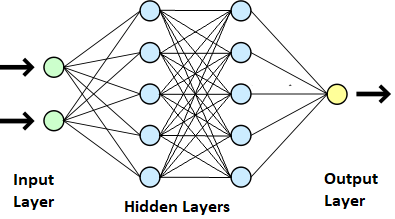
\includegraphics[width=0.95\linewidth]{images/learn_levelset/MLP_schema.png}
	\end{minipage}
	
	\vspace{5pt}
	
	\textbf{DoFs Minimization Problem :} \\
	Considering the least-square form of (\ref{edp}), our discrete problem is
	\begin{equation*}
		\displaystyle \theta_u=\argmin_{\theta\in\mathbb{R}^N} \alpha J_{in}(\theta)+\beta J_{bc}(\theta) %\label{minpb_pinns}
	\end{equation*}
	with $N$ the number of parameters of the NN and
	\begin{equation*}
		J_{in}(\theta)=\frac{1}{2}\int_\Omega (L(u_\theta) - f)^2  \qquad \text{and} \qquad J_{bc}(\theta)=\frac{1}{2}\int_{\partial\Omega} (u_\theta-g)^2
	\end{equation*}	
	
	\textbf{Monte-Carlo method :} Discretize the cost function by random process.
\end{frame}

\begin{frame}{Limits}
	\textbf{Claim on PINNs :} \textcolor{orange}{No mesh, so easy to go on complex geometry !}
	
	\warning \textit{In practice :} Not so easy ! We need to find \textcolor{orange}{how to sample in the geometry}.
	
	\vspace{8pt}
	
	\textbf{Solution :} Approach by levelset.
	
	\begin{center}
		\pgfimage[width=0.4\linewidth]{images/learn_levelset/levelset.png}
	\end{center}
	
	\vspace{5pt}

	\begin{center}
		\begin{minipage}{0.44\linewidth}
			\textbf{\textit{Advantages :}} \\
			\ding{217} Sample is easy in this case. \\
			\ding{217} Allow to impose in hard the BC :
			\vspace{-5pt}
			\begin{equation*}
				u_\theta(X)=\phi(X)w_\theta(X)+g(X)
			\end{equation*}
		\end{minipage}
		\begin{minipage}{0.44\linewidth}
			\textbf{\textit{Natural LevelSet :}} \\
			Signed Distance Function (SDF)
			
			\vspace{5pt}
			\textbf{\textit{Problem :}} SDF is a $\mathcal{C}^0$ function  \\
			$\Rightarrow$ its derivatives explode \\
			$\Rightarrow$ we \textcolor{orange}{need a regular levelset}
		\end{minipage}
	\end{center}
\end{frame}

\begin{frame}{Learn a regular levelset}	
	\vspace{-10pt}
	\begin{tcolorbox}[
		colback=other, % Couleur de fond de la boîte
		colframe=other, % Couleur du cadre de la boîte
		arc=2mm, % Rayon de l'arrondi des coins
		boxrule=0.5pt, % Épaisseur du cadre de la boîte
		breakable, enhanced jigsaw,
		width=\linewidth,
		opacityback=0.1
		]
		
		If we have a boundary domain $\Gamma$, the SDF is solution to the Eikonal equation:
		
		\begin{minipage}{\linewidth}
			\centering
			$\left\{\begin{aligned}
				&||\nabla\phi(X)||=1, \; X\in\mathcal{O} \\
				&\phi(X)=0, \; X\in\Gamma \\
				&\nabla\phi(X)=n, \; X\in\Gamma
			\end{aligned}\right.$
		\end{minipage}
		
		with $\mathcal{O}$ a box which contains $\Omega$ completely and $n$ the exterior normal to $\Gamma$.
	\end{tcolorbox}

	\textbf{How to do that ?} with a PINNs \cite{clemot_neural_2023} by \textcolor{orange}{adding a regularization term}.
	\vspace{-5pt}
	\begin{equation*}
		J_{reg} = \int_\mathcal{O} |\Delta\phi|^2
	\end{equation*}

	\begin{minipage}{0.32\linewidth}
		\centering
		\pgfimage[width=\linewidth]{images/learn_levelset/cat_levelset_loss.png}
	\end{minipage} 
	\begin{minipage}{0.32\linewidth}
		\centering
		\pgfimage[width=\linewidth]{images/learn_levelset/cat_levelset.png}
	\end{minipage} 
	\begin{minipage}{0.32\linewidth}
		\centering
		\pgfimage[width=\linewidth]{images/learn_levelset/cat_levelset_bc.png}
	\end{minipage} 
\end{frame}

\begin{frame}{Poisson On Cat}	
	\ding{217} Solving the \textcolor{orange}{Poisson problem} with $f=1$ and homogeneous Dirichlet BC. \\
	\ding{217} Looking for $u_\theta = \phi w_\theta$ with $\phi$ the levelset learned. 
	
	\begin{center}
		\begin{minipage}{0.32\linewidth}
			\textbf{Sampling}
			
			\vspace{-10pt}
			\centering
			\pgfimage[width=0.6\linewidth]{images/learn_levelset/cat_levelset_sampling.png}
		\end{minipage} \qquad 
		\begin{minipage}{0.32\linewidth}
			\centering
			\pgfimage[width=\linewidth]{images/learn_levelset/cat_poisson_loss.png}
		\end{minipage} 
	\end{center}

	\begin{center}
		\pgfimage[width=0.8\linewidth]{images/learn_levelset/cat_poisson_sol.png}
	\end{center}

	\footnotesize
	\textit{Remark :} Poisson on Bean \refappendix{frame:bean}
\end{frame}